% <!-- This makes it look pretty in a browser --><pre>
\documentclass[a4paper,english]{cv}
\usepackage[latin1]{inputenc}
\usepackage{a4wide}
\pagestyle{empty}
\usepackage{graphicx}
\usepackage{longtable}
\makeatletter
\newcommand{\HS}{\hspace{0.5cm}}
\date{}
\newcommand{\B}[1]{%
\makebox[1cm][l]{\small{#1:}}}
\newcommand{\VT}{\vspace{2mm}}
\renewcommand{\topicmargin}{7em}
\usepackage{babel}
\makeatother
\begin{document}
\title{Curriculum Vitae}
\maketitle
\thispagestyle{empty}\centerline{\fbox{\begin{minipage}[c]{0.50\columnwidth}%
\begin{center}\hfill{}\hfill{}\begin{tabular}{p{2.1cm}p{4cm}}
Name:&
Martin Strauss\\
Address:&
\parbox[t]{4cm}{Karcherstra�e 16
\\
66111 Saarbr�cken
\\
GERMANY\VT{}}\\
Telephone:&
\parbox[t]{4cm}{Home: +49 681 5006 376
\\
Mobile: +49 163 1462 550\VT{}}\\
E-mail:& martin@ockle.org\\
Birth:& 19th July, 1983; K�ln, Germany\\
Citizenship:& Australian (naturalised 26th January 1988)\\
\end{tabular}\hfill{}\end{center}\end{minipage}%
\begin{minipage}[c]{0.50\columnwidth}%
~\hfill{}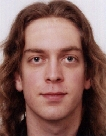
\includegraphics[%
  width=0.50\columnwidth,
  keepaspectratio]{Strauss_Martin.jpg}\hfill{}~\end{minipage}%
}}
\section{Skills}
\subsection{Computer Skills}

\begin{topic}
\item [ OS]  Expert user of Unix (especially Linux and SunOS) and Mac OS X, advanced user of Windows.

\item [ Languages]  Extensive experience with C, Java, C++, Prolog, Javascript, PHP, Python and Perl, as well as BASH shell scripting. Also experience with languages such as Haskell, Lex/Yacc, BASIC, RSI IDL and Assembler (primarily x86) as well as some exposure to Pascal, Scheme, Lisp, etc.

\item [ Software Engineering]  Extensive experience with UML and Object-Oriented design, agile development methods, and also with functional and logic programming.  Also experience with Microsoft Visual Studio, Rational Rose, Eclipse, NetBeans.

\item [ Administration]  Extensive experience administering Linux servers (primarily Debian GNU/Linux and Gentoo, but also Red Hat, Mandrake and Slackware), and some experience administering Windows NT4, 2000 and XP workstations and Windows NT4, 2000 and 2003 servers. Experience with directory services (LDAP), SQL databases (MySQL and PostgreSQL), firewalls and routing (netfilter/iptables and ipfilter), Internet proxy services (squid, dante-socks), mail services (sendmail, exim, postfix), etc.

\item [ Tools]  Experience using and programming MATLAB and RSI IDL, and toolboxes such as Simulink.

\end{topic}
\subsection{Language Skils}

\begin{topic}
\item [ English]  native language

\item [ German]  native language

\item [ Japanese]  some knowledge

\end{topic}
\section{Employment}

\begin{topic}
\item [2007 --] \textbf{Software Engineer, Google Inc.}  Freigutstrasse 12, CH-8002 Z�rich, Switzerland

\item [2006 -- 2007] \textbf{Research Assistant, Deutsche Forschungszentrum f�r K�nstliche Intelligenz}  Stuhlsatzenhausweg 3 (Geb�ude D3 2)
D-66123 Saarbr�cken, Germany

\item [2006] \textbf{Software Engineer, Defence Science and Technology Organisation}  506 Lorimer St, Fishermans Bend VIC 3207, Australia

\item [2005] \textbf{Tutor, Ormond College}  College Crescent, Parkville, VIC 3052, Australia

\item [2004 -- 2005] \textbf{Software Engineering Project and Advanced Software Engineering Project}  

\item [2001 -- 2005] \textbf{IT Administrator, Ormond College}  College Crescent, Parkville, VIC 3052, Australia

\item [Summer 1999, 2000] \textbf{Laboratory Assistant, Rohm and Haas Australia Pty. Ltd.}  Hays Road, Point Henry, Geelong, VIC 3220, Australia

\end{topic}

\section{Education}

\begin{topic}
\item [2006 -- 2007]\textbf{Master of Science} The University of Saarland and Max Planck Institute for Computer Science\item [2004 -- 2005]\textbf{Taste of Research Summer Scholarship} The University of New South Wales and National ICT Australia\item [2001 -- 2005]\textbf{Bachelor of Engineering (Software), Diploma of
    Music (Practical)} The University of Melbourne\item [1999 -- 2000]\textbf{Melbourne University Program for High Achieving Students} The University of Melbourne\item [1999 -- 2000]\textbf{International Baccalaureate} Geelong Grammar School\item [1994 -- 2000]\textbf{Geelong Grammar School} \item [1989 -- 1993]\textbf{The Geelong College} \end{topic}

\section{Other Training}

\begin{topic}
\item [December 2004] The Australian Logic Summer School

\item [February 2002] SecureCON

\item [April 2000] Australian Business Week

\end{topic}
\section{Other positions held}

\begin{topic}
\item [2003] \textbf{Head of Pleasant Sunday/Wednesday Evening Subcommittee of the Ormond College Students' Club}

\item [2003 -- 2005] \textbf{Senior Chorister, the Choir of Ormond College}

\item [2000] \textbf{School Music captain, Geelong Grammar School}

\end{topic}

\end{document}
%</pre><!-- This makes it look pretty in a browser -->
